% Space beam element lying along the global Y axis, with four choices of y'
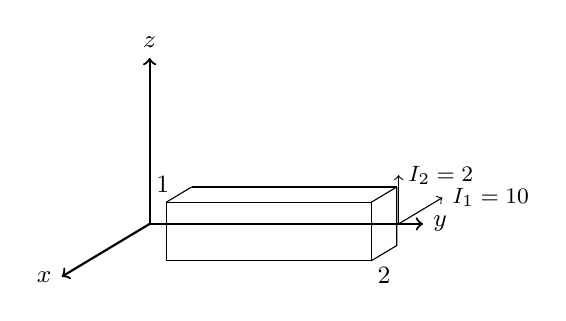
\begin{tikzpicture}[scale=0.62,font=\small,x={(-0.75cm,-0.45cm)},y={(1cm,0cm)},z={(0cm,1cm)}]
  % axes
  \draw[->,thick] (0,0,0) -- (2.4,0,0) node[left] {$x$};
  \draw[->,thick] (0,0,0) -- (0,5.6,0) node[right] {$y$};
  \draw[->,thick] (0,0,0) -- (0,0,3.4) node[above] {$z$};
  % member box from y=0.4 to y=5 with section 0.5 (x) by 1.0 (z)
  \def\ya{0.6} \def\yb{4.8} \def\hx{0.35} \def\hz{0.6}
  \draw (\hx,\ya,\hz) -- (\hx,\yb,\hz) -- (\hx,\yb,-\hz) -- (\hx,\ya,-\hz) -- cycle;
  \draw (-\hx,\ya,\hz) -- (-\hx,\yb,\hz); \draw (\hx,\ya,\hz) -- (-\hx,\ya,\hz); \draw (\hx,\yb,\hz) -- (-\hx,\yb,\hz);
  \draw (-\hx,\yb,\hz) -- (-\hx,\yb,-\hz) -- (\hx,\yb,-\hz);
  \draw[dashed] (0,\ya,0) -- (0,\yb,0);
  \node[left] at (0,\ya,\hz+0.2) {1}; \node[below] at (0,\yb,-\hz-0.1) {2};
  \draw[->] (0,\yb+0.3,0) -- (0,\yb+0.3,1.0) node[right,font=\footnotesize] {$I_2 = 2$};
  \draw[->] (0,\yb+0.3,0) -- (-1.2,\yb+0.3,0) node[right,font=\footnotesize] {$I_1 = 10$};
\end{tikzpicture}
